\subsection{Glyph: \glyph{Unit of information for Biological activity}}
\label{sec:af:unitInfo}

When representing biological activities, it is often useful to illustrate the nature of the entity where the activity is originated, eg., whether the activity is from a macromolecule (protein or nucleic acid), or from a chemical compound.  The \SBGNAFLone \glyph{unit of information} is used to add such information to a glyph.  It represents the information in two ways.  First, different symbols are used to represent the nature of the entity where the activity is from, e.g.., macromolecule, nucleic acid feature, or complex.  These symbols are identical to the \glyph{entity pool node} symbols in SBGN \PDl.  Second, names of the entity (gene names, protein names) are usually provided as labels in the \glyph{unit of information} container.

\begin{glyphDescription}

\glyphSboTerm Not applicable.

\glyphContainer A unit of information is represented by containers of different shapes, depending on the nature of the entity where the biological activity is from. There are a total of five types of unit of information, as shown in \fig{af:unitInfo}.   Below is a summary of the five glyphs.

\begin{description}
\item[A.] macromolecule -- Macromolecules are biochemical substances that are built up from the covalent linking of pseudo-identical units. Examples of macromolecules include proteins, nucleic acids (RNA, DNA), and polysaccharides (glycogen, cellulose, starch, etc.).  
A unit of information of a macromolecule is represented by a rectangle with rounded corners, as illustrated in (A) of \fig{af:unitInfo}.  This container is used to decorate a biological activity that is originated from a macromolecule, such as a protein, a nucleic acid, or a complex sugar.

\item[B.] nucleic acid feature -- The Nucleic acid feature construct in SBGN is meant to represent a fragment of a macromolecule carrying genetic information. A unit of information of a nucleic acid feature is represented by a rectangle whose bottom half has rounded corners, as shown in (B) of  \fig{af:unitInfo}.

\item[C.] simple chemical -- A simple chemical is a chemical compound that is not formed by the covalent linking of pseudo-identical residues. Examples of simple chemicals are an atom, a monoatomic ion, a salt, a radical, a solid metal, a crystal, etc. 
A unit of information of a simple chemical is represented by a circular container, as shown in (C) of \fig{af:unitInfo}.

\item[D.] unspecified entity -- An unspecified entity is used to represent the entity type that is unknown or simply not relevant to the purposes of the map. This arises, for example, when the existence of the entity has been inferred indirectly, or when the entity is merely a construct introduced for the needs of a map, without direct biological relevance. A unit of information of an unspecified entity is represented by an elliptic container, as shown in (D) of \fig{af:unitInfo}.  It is used to decorate a biological activity that is originated from an unspecified entity.

\item[E.] complex -- A complex represents a biochemical entity composed of other biochemical entities, whether macromolecules, simple chemicals, or other complexes. The resulting entity may 
have its own identity, properties and function in an SBGN map. A unit of information of a complex is represented by an octagon as shown in (E) of \fig{af:unitInfo}.  It is used to decorate a biological activity that is originated from a complex.
\end{description}

\begin{figure}[H]
  \centering
  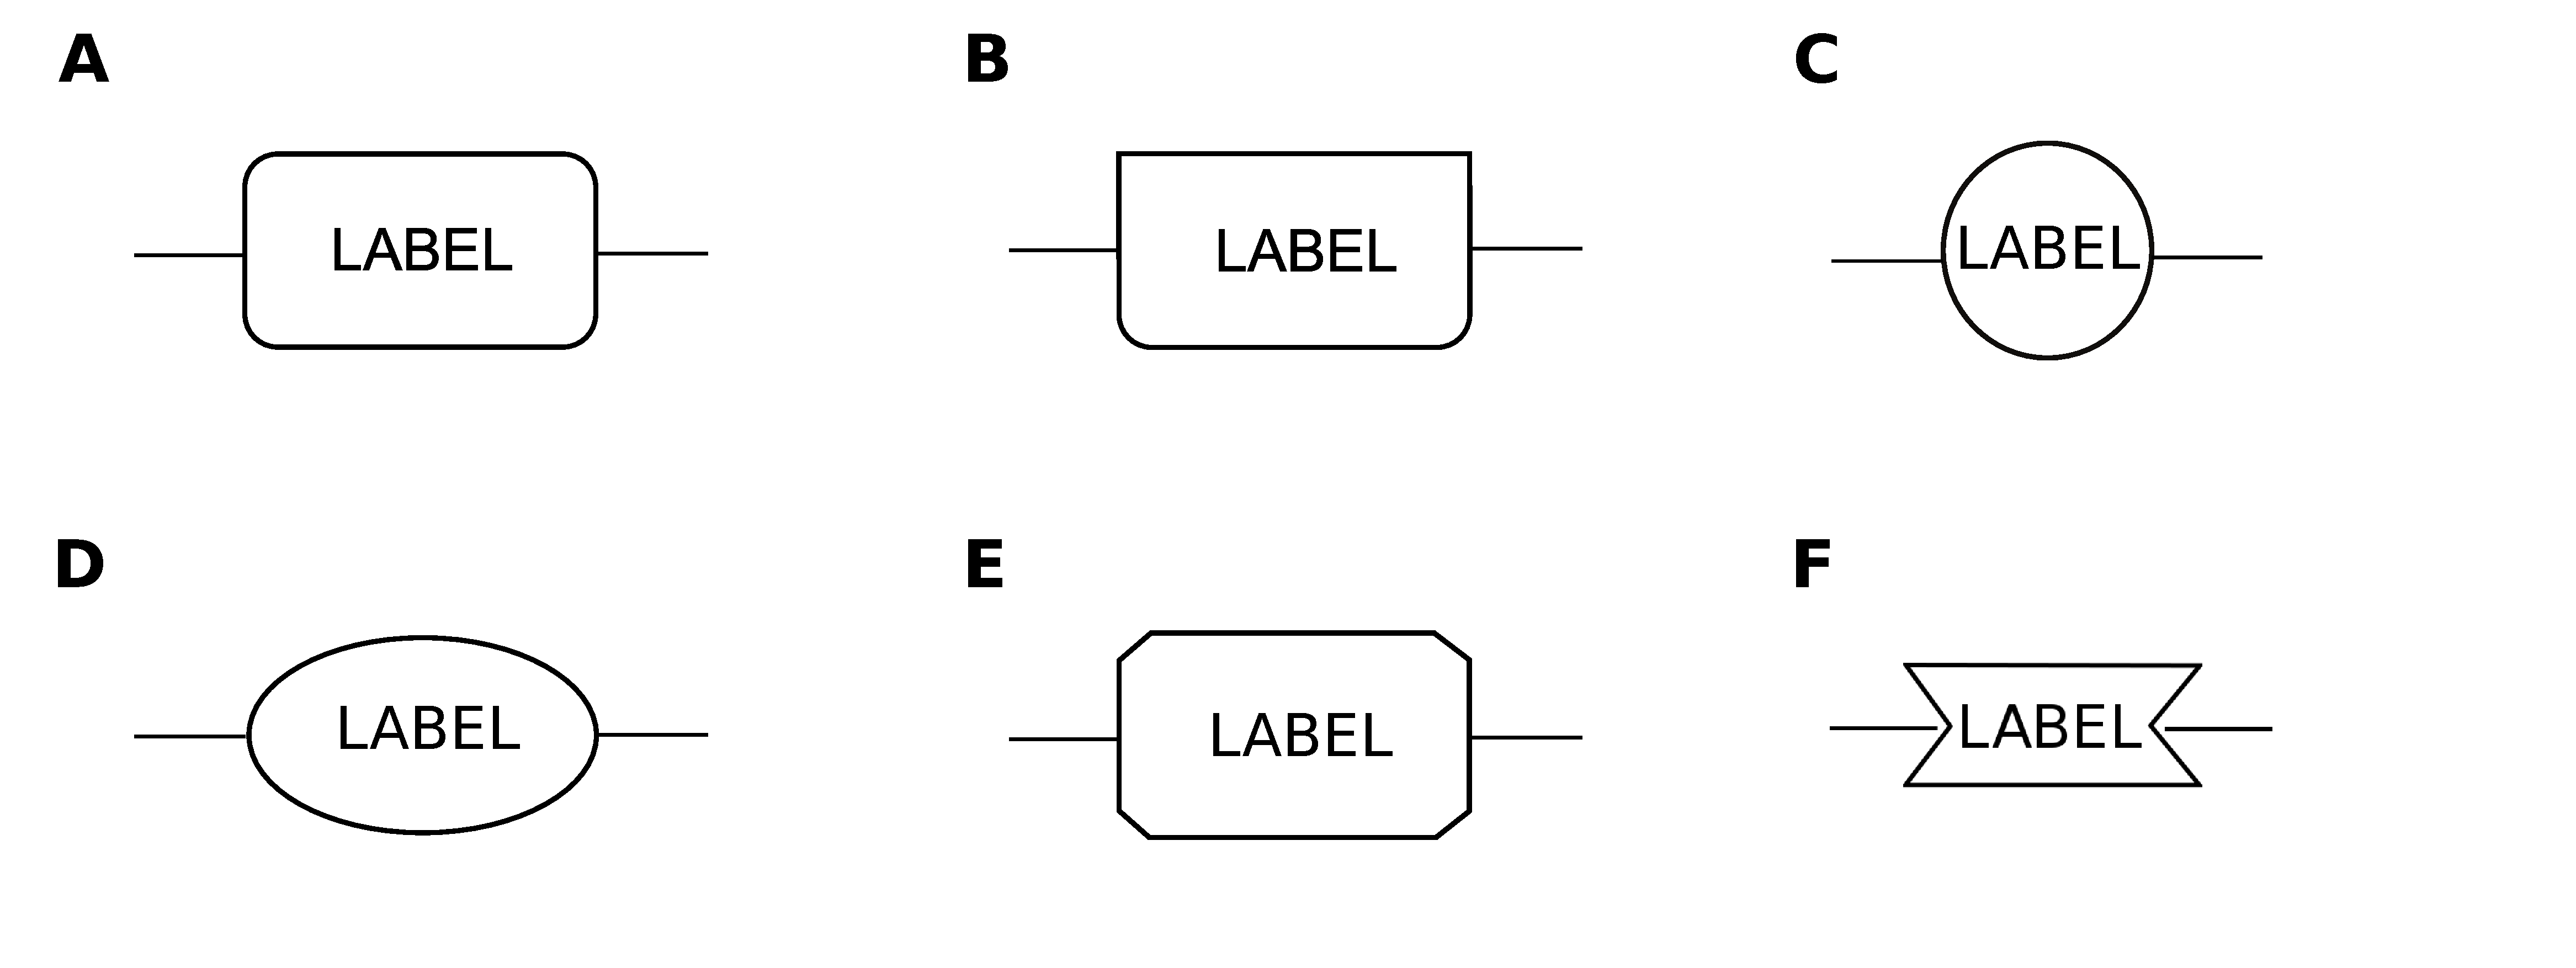
\includegraphics[scale = 0.2]{images/unitInformation_ba}
  \caption{The \AF glyph for \glyph{unit of information}.}
  \label{fig:af:unitInfo}
\end{figure}

\begin{figure}[H]
  \centering
  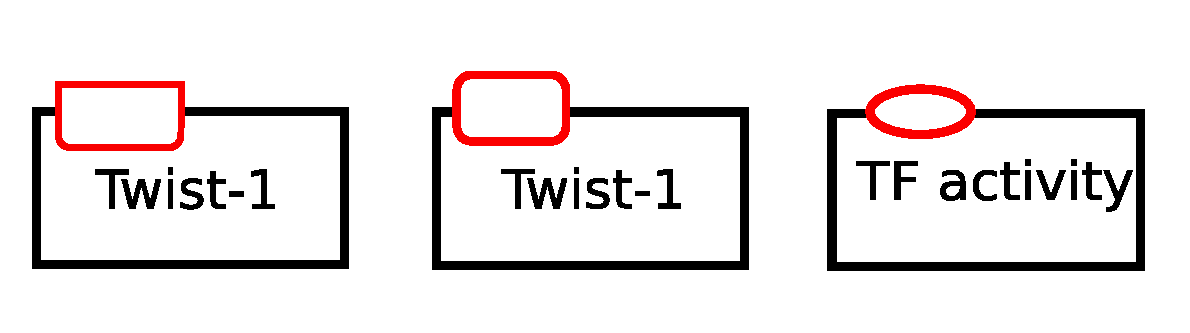
\includegraphics[scale = 0.5]{examples/unitofinformation}
  \caption{Examples of \glyph{unit of information} used on \glyph{biological activity node} to indicate that the \emph{Twist-1 activity} is from a \emph{nucleic acid feature} or a \emph{macromolecule}, or a \emph{transcription factor activity} from an \emph{unspecified} entity.}
  \label{fig:af:unitofinfo}
\end{figure}

\fig{af:unitofinfo} shows examples taken from \fig{af:1}, where \emph{units of information} is used on Activity Nodes to illustrate the properties of the entities that the activities are originated from.

The long side of the glyphs above (except for simple chemical) should be oriented parallel to the border of the \glyph{AN} being annotated by the \glyph{unit of information}. The center of the bounding box of a \glyph{state of information} should be located on the mid-line of the border of the \glyph{AN}.

\glyphLabel A \glyph{unit of information} is not required to carry any label.   If a label is desired, it should be placed in an unbordered box containing a string of characters. The characters can be distributed on several lines to improve readability, although this is not mandatory.  The label box must be attached to the center of the container. The label may spill outside of the container.  The label defines the information carried by the \glyph{unit of information}.

\glyphAux A \glyph{unit of information} does not carry any auxiliary items.

\end{glyphDescription}

\subsection{Glyph: \glyph{Unit of information for Compartment}}
\label{sec:af:unitInfoComp}

A \emph{unit of information} can be used to decorate a compartment to convey information about physical characteristics of the compartments (\sect{af:physical-characteristics-cv}). 

\begin{glyphDescription}

\glyphSboTerm Not applicable.

\glyphContainer A \emph{unit of information} for compartment is represented by a rectangle as shown in \fig{compunitInfo}.  The long side of the rectangle should be oriented parallel to the border of the \glyph{compartment} being annotated by the \glyph{unit of information}. The center of the bounding box of a \glyph{state of information} should be located on the mid-line of the border of the \glyph{compartment}.

\begin{figure}[H]
  \centering
  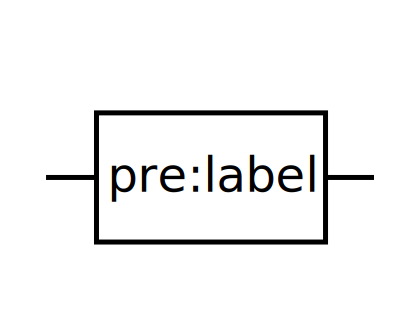
\includegraphics[scale = 0.5]{images/unitInformation}
  \caption{The \AF glyph for \glyph{unit of information}.}
  \label{fig:compunitInfo}
\end{figure}

\glyphLabel A \glyph{unit of information} is identified by a label placed in an unbordered box containing a string of characters.  The characters can be distributed on several lines to improve readability, although this is not mandatory.  The label box must be attached to the center of the container.  The label may spill outside of the container.

The label defines the information carried by the \glyph{unit of information}.  For certain predefined types of information for the compartment, such as physical characteristics, SBGN defines specific prefixes that must be included in the label to indicate the type of information in question.  The controlled vocabularies predefined in \SBGNAFLone are described in \sect{af:physical-characteristics-cv} and summarized in the following list:

\begin{center}
  \begin{itemize}\setlength{\parskip}{0ex}
  \item[\texttt{pc:T}] Temperature (SBO:0000147)
  \item[\texttt{pc:V}] Voltage (SBO:0000259)
  \item[\texttt{pc:pH}] pH (SBO:0000304)
  \end{itemize}
\end{center}

    
\glyphAux A \glyph{unit of information} does not carry any auxiliary items.  

\end{glyphDescription}


